\documentclass[11pt]{article} 

\usepackage[utf8]{inputenc} 

\usepackage{graphicx}

\usepackage{geometry}
\geometry{a4paper} 


\title{Winterthur Yard: Zwischenstand Projekt}
\author{Maja Fritschi, Raphael Spörri, Florian Bosshard}
\date{} 
\begin{document}
\maketitle

\tableofcontents
\newpage

\section{Projektteam}
Das Projekt wird von folgenden Personen entwickelt:
\begin{itemize}
\item Maja Fritschi (fritsmaj)
\item Raphael Spörri (sporrra0)
\item Florian Bosshard (bosshflo)
\end{itemize}


\section{Umgesetzte Funktionalitäten}
Folgend werden Funktionalitäten aufgelistet die bis zum 6. November 2013 umgesetzt wurden: 
\begin{itemize}
\item Datenbank mit den entsprechneden Tabellen ist aufgesetzt, sowie mit Koordinatenpunkten befüllt.
\item Anmelde-Screan wo man mit der Angabe des Namens sich für das Spiel einloggen kann. Der Name wird zum Server gesendet und in der Datenbank gespeichert. Eine neue Session wird gestartet.
\item Die Koordinatenpunkte werden auf der Karte eingezeichtet und mit Linien verbunden. Es können auch Zwischenpunkte gesetzt werden, damit die Koordinatenunkt nicht nur mit geraden Linien verbunden werden können.
\item Die Logik, dass sich MisterX automatisch bewegt ist implementiert.
\item Mit einem Klick auf den Button ``Catch me!'' wird die aktuelle Position des Spielers ermittelt und an den Server geschickt. Der Spieler erhält dann die Nachricht, ob er den MisterX gefangen hat, ob nicht oder ob er keinem Koordinatenpunkt auf der Karte zugewiesen werden konnte.
\end{itemize}

Die aktuelle Applikation kann unter yard.prusik.ch angeschaut werden. 

\section{Aufgetretene Probleme}
Wir haben anfangs versucht mit jQueryMobile 1.4 zu arbeiten, sind dann aber auf Probleme beim Einbetten der Karte gestossen. Daher haben wir zurück auf jQueryMobile 1.3 gewechselt.


\section{Offene Funktionalitäten}
\begin{itemize}
\item MisterX und die Spieler auf der Karte anzeigen.
\item Side-Menu zur Navigation mit den Einträgen Hilfe und About.
\item Spiel und Session beenden sowie Aufräumen der Datenbank ausprogrammieren.
\item Mehr Punkte auf der Karte erfassen.
\item Das GUI muss noch via einem Theme angepasst werden, damit die Applikation kein Standard-Aussehen hat.
\item Finale Messages nach dem Drücken auf den ``Cach Me!''-Button erstellen.
\item Spiel testen
\end{itemize}
 

\section{Screenshots}
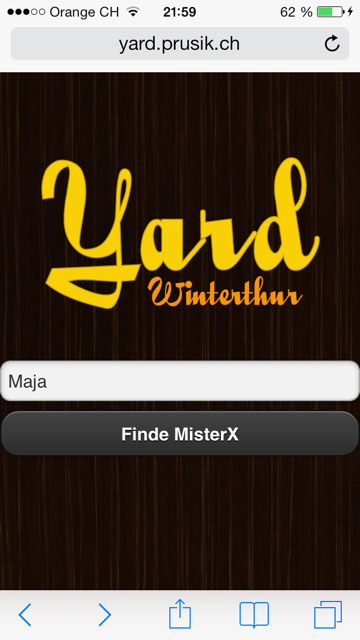
\includegraphics[width=8cm]{Bilder/HomeScreen.jpg}
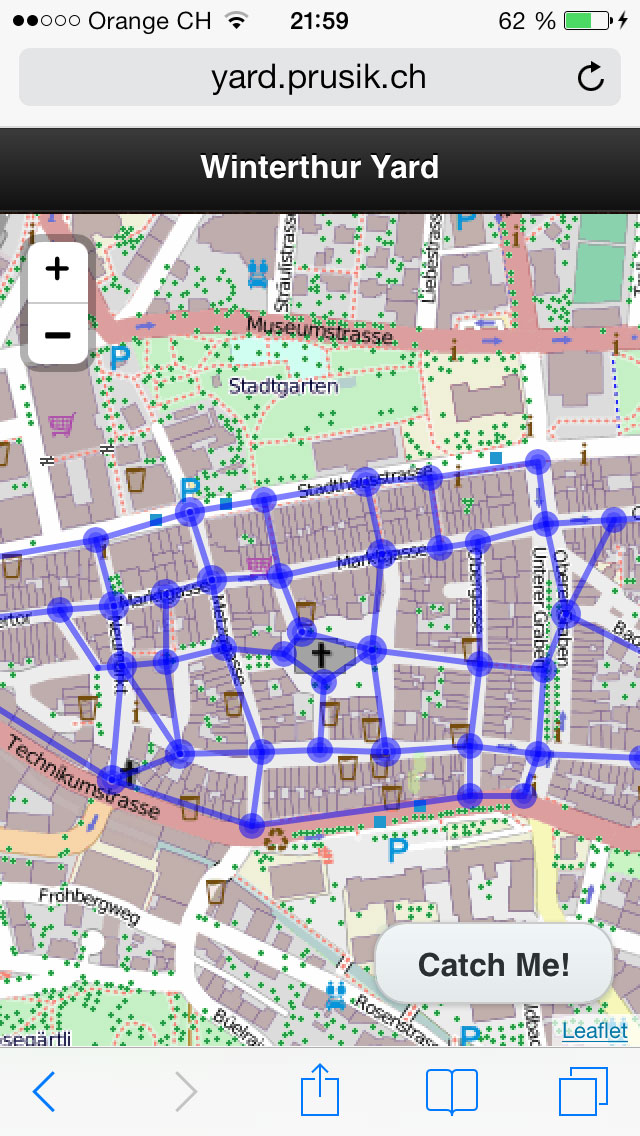
\includegraphics[width=8cm]{Bilder/Karte.jpg}
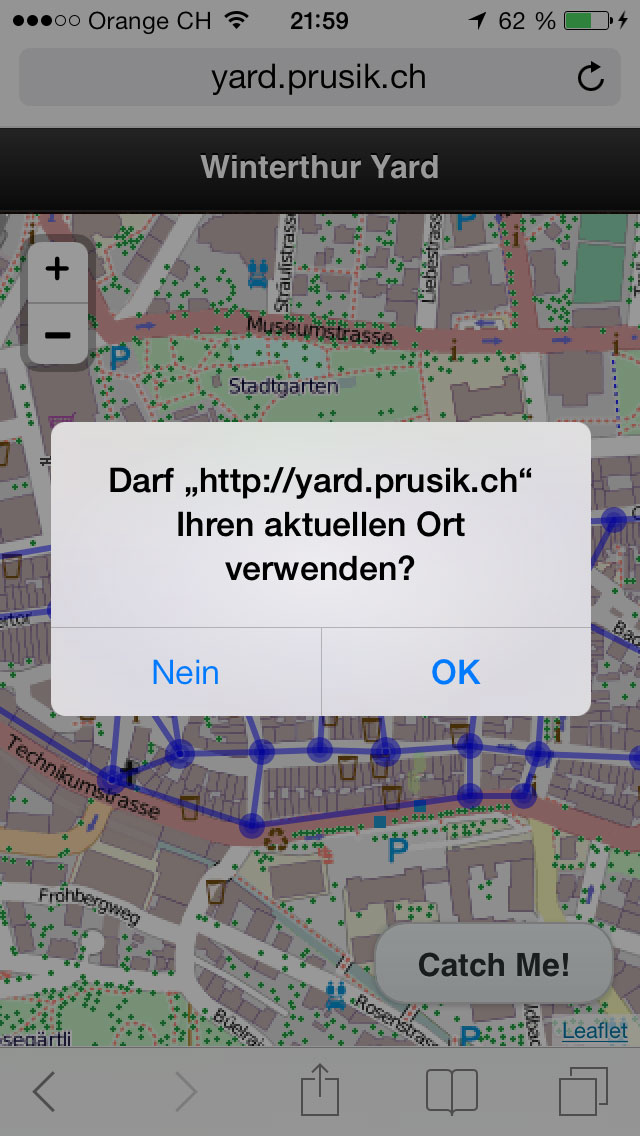
\includegraphics[width=8cm]{Bilder/Position.jpg}
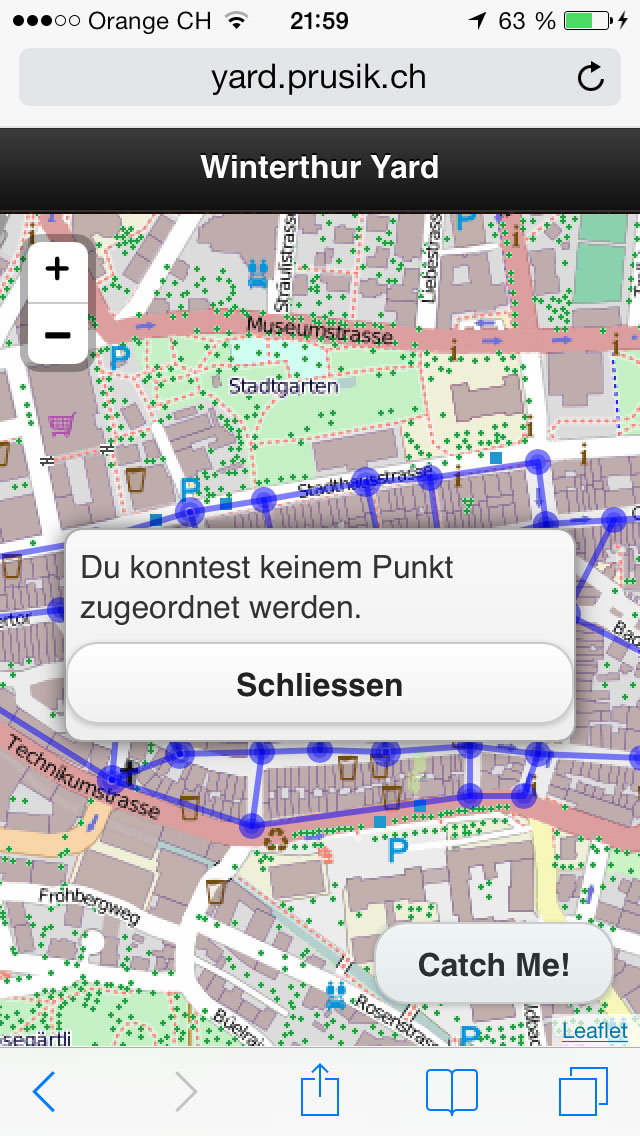
\includegraphics[width=8cm]{Bilder/KeinePosition.jpg}


Wenn MisterX nicht gefunden wurde, wird seine letzte Position mit einem roten Kreis dargestellt:  \\
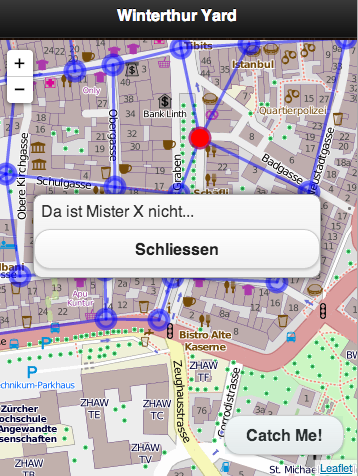
\includegraphics[width=8cm]{Bilder/notFound.png}

Sowohl der Graph als auch die Anfrage werden über eine REST-Api über JSON übertragen \\
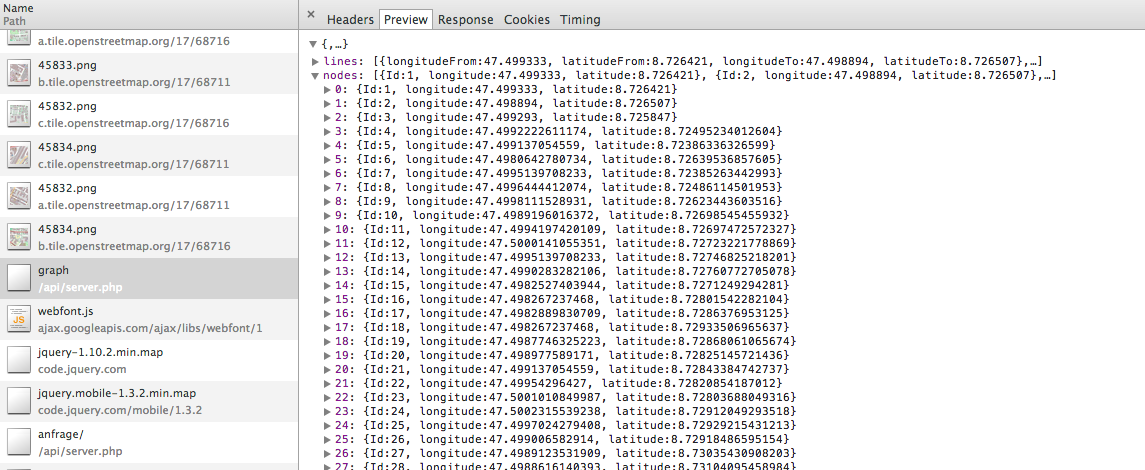
\includegraphics[width=15cm]{Bilder/rest.png}


\end{document}
